\documentclass[12pt]{book}

\newcommand{\thetitle}{Think Java: How to Think Like a Computer Scientist}
\title{\thetitle}

\newcommand{\theauthors}{Allen Downey and Chris Mayfield}
\author{\theauthors}

\newcommand{\theversion}{Version 6.0 Draft -- \today}
\date{\theversion}

\usepackage{geometry}
\geometry{
    width=5.5in,
    height=8.5in,
    hmarginratio=3:2,
    vmarginratio=1:1,
    includehead=true,
    headheight=15pt
}

% paragraph spacing
\setlength{\parindent}{0pt}                      % 17.62482pt
\setlength{\parskip}{12pt plus 4pt minus 4pt}    % 0.0pt plus 1.0pt
\linespread{1.05}
\def\arraystretch{1.5}

% list spacing
\setlength{\topsep}{5pt plus 2pt minus 3pt}      % 10.0pt plus 4.0pt minus 6.0pt
\setlength{\partopsep}{-6pt plus 2pt minus 2pt}  %  3.0pt plus 2.0pt minus 2.0pt
\setlength{\itemsep}{0pt}                        %  5.0pt plus 2.5pt minus 1.0pt

% these are copied from tex/latex/base/book.cls
% all I changed is afterskip
\makeatletter
\renewcommand{\section}{\@startsection {section}{1}{\z@}%
    {-3.5ex \@plus -1ex \@minus -.2ex}%
    {0.7ex \@plus.2ex}%
    {\normalfont\Large\bfseries}}
\renewcommand\subsection{\@startsection{subsection}{2}{\z@}%
    {-3.25ex\@plus -1ex \@minus -.2ex}%
    {0.3ex \@plus .2ex}%
    {\normalfont\large\bfseries}}
\renewcommand\subsubsection{\@startsection{subsubsection}{3}{\z@}%
    {-3.25ex\@plus -1ex \@minus -.2ex}%
    {0.3ex \@plus .2ex}%
    {\normalfont\normalsize\bfseries}}
\makeatother

% table of contents vertical spacing
\usepackage{tocloft}
\setlength\cftparskip{8pt plus 4pt minus 4pt}

% The following line adds a little extra space to the column
% in which the Section numbers appear in the table of contents
\makeatletter
\renewcommand{\l@section}{\@dottedtocline{1}{1.5em}{3.0em}}
\makeatother

% customize page headers
\usepackage{fancyhdr}
\pagestyle{fancyplain}
\renewcommand{\chaptermark}[1]{\markboth{Chapter \thechapter ~~ #1}{}}
\renewcommand{\sectionmark}[1]{\markright{\thesection ~~ #1}}
\lhead[\fancyplain{}{\bfseries\thepage}]%
      {\fancyplain{}{\bfseries\rightmark}}
\rhead[\fancyplain{}{\bfseries\leftmark}]%
      {\fancyplain{}{\bfseries\thepage}}
\cfoot{}
%\rfoot{\textcolor{gray}{\tiny ThinkJava Draft \today}}

% balanced index with TOC entry
\usepackage{makeidx}
\makeindex
%\usepackage[totoc]{idxlayout}

% automatically index glossary terms
\newcommand{\term}[1]{%
\index{#1}
\item[#1:]}
% TODO: doesn't work with plastex
%\newcommand{\term}[1]{\item[#1:]}

% where to find graphics
\usepackage{graphicx}
%\graphicspath{{figs/}}

%% tweak spacing of figures and captions
%\usepackage{floatrow}
%\usepackage{caption}
%\captionsetup{
%    font=small,
%    labelformat=empty,
%    justification=centering,
%    skip=4pt
%}

% format end of chapter excercises
\usepackage{amsmath}
\usepackage{amsthm}
\newtheoremstyle{exercise}
  {12pt}        % space above
  {12pt}        % space below
  {}            % body font
  {}            % indent amount
  {\bfseries}   % head font
  {}            % punctuation
  {12pt}        % head space
  {}            % custom head
\theoremstyle{exercise}
\newtheorem{exercise}{Exercise}[chapter]

% colors for code listings and output
\usepackage{xcolor}
\definecolor{bgcolor}{HTML}{FAFAFA}
\definecolor{comment}{HTML}{007C00}
\definecolor{keyword}{HTML}{0000FF}
\definecolor{strings}{HTML}{B20000}

% syntax highlighting in code listings
\usepackage{textcomp}
\usepackage{listings}
\lstset{
    language=java,
    basicstyle=\ttfamily,
    backgroundcolor=\color{bgcolor},
    commentstyle=\color{comment},
    keywordstyle=\color{keyword},
    stringstyle=\color{strings},
    columns=fullflexible,
    keepspaces=true,
    showstringspaces=false,
    upquote=true,
    aboveskip=\parskip,
    belowskip=\parskip
}

% code listing environments
\lstnewenvironment{code}
{\minipage{\linewidth}}
{\endminipage}
\lstnewenvironment{stdout}
{\lstset{commentstyle=,keywordstyle=,stringstyle=}\minipage{\linewidth}}
{\endminipage}

% pdf hyperlinks, table of contents, and document properties
\usepackage[pdftex]{hyperref}
\hypersetup{%
  pdftitle={\thetitle},
  pdfauthor={\theauthors},
  pdfsubject={\theversion},
  pdfkeywords={},
  bookmarksopen=false,
  colorlinks=true,
  citecolor=black,
  filecolor=black,
  linkcolor=black,
  urlcolor=blue
}

% inline syntax formatting
\newcommand{\java}[1]{\lstinline{#1}} %\end{
%\newcommand{\java}[1]{\verb"#1"}
%\newcommand{\java}[1]{{\tt #1}}

\begin{document}
\setcounter{chapter}{5}

\chapter{Value methods}

Some of the methods we have been using, like the \java{Math} methods, return values.
Other methods, like \java{println} and \java{newLine}, perform an action but they don't return a value.
That raises some questions:

\begin{itemize}

\item What happens if you invoke a method and you don't do anything with the result?
(In other words, if you don't assign it to a variable or use it as part of a larger expression?)

\item What happens if you use a \java{print} method as part of an expression?
For example: \java{System.out.println("boo!") + 7;}

\item Can we write methods that return values, or are we stuck with things like \java{newLine} and \java{printTwice}?

\end{itemize}

The answer to the third question is yes, and that is the focus of this chapter.
It's up to you to answer the other two questions by trying them out.
In fact, any time you have a question about what is legal or illegal in Java, a good way to find out is to ask the compiler.
%If you're using DrJava, you can quickly try out these examples in the Interactions Pane.


\section{Return values}

\index{void}
\index{method!void}

The simple methods we have written in previous chapters are \java{void}.
In other words, they are a sequence of statements that return no value.
When you invoke a \java{void} method, it is typically on a line all by itself:

\begin{code}
    countdown(3);
    System.out.println("Have a nice day.");
\end{code}

In contrast, some of the methods we have used produce results.
That is, the effect of invoking the method is to generate a new value, which we usually assign to a variable or use as part of an expression:

\begin{code}
    double error = Math.abs(expected - actual);
    double height = radius * Math.sin(angle);
\end{code}

\index{value method}
\index{method!value}

In this chapter, you will learn to write methods that \java{return} values.
The first example is \java{area}, which takes a \java{double} as a parameter and returns the area of a circle with that radius:

\begin{code}
    public static double area(double radius) {
        double area;
        area = Math.PI * radius * radius;
        return area;
    }
\end{code}

The first thing you should notice is that the beginning of the method definition is different.
Instead of \java{public static void}, which indicates a \java{void} method, we see \java{public static double}, which means that the return value from this method is a \java{double}.
%I still haven't explained what {\tt public static} means, but be patient.

\index{return}
\index{statement!return}

The last line is a new form of the \java{return} statement that includes a return value.
This statement means, ``return immediately from this method and use the following expression as the return value.''
The expression you provide can be arbitrarily complex, so we could have written this method more concisely:

\begin{code}
    public static double area(double radius) {
        return Math.PI * radius * radius;
    }
\end{code}

\index{temporary variable}
\index{variable!temporary}

On the other hand, {\bf temporary} variables like \java{area} often make debugging easier, especially when you are stepping through code using an integrated debugger.
In either case, the type of the expression in the \java{return} statement must match the return type of the method.
When you declare that the return type is \java{double}, you are making a promise that this method will eventually produce a \java{double} value.
If you try to \java{return} with no expression, or an expression with the wrong type, the compiler will give an error.

Sometimes it is useful to have multiple return statements, for example, one in each branch of a decision:

\begin{code}
    public static double absoluteValue(double x) {
        if (x < 0) {
            return -x;
        } else {
            return x;
        }
    }
\end{code}

Since these \java{return} statements are in an alternative structure, only one will be executed.
Although it is legal to have more than one \java{return} statement in a method, you should keep in mind that as soon as one is executed, the method terminates without executing any subsequent statements.

\index{dead code}

Code that appears after a \java{return} statement, or any place else where it can never be executed, is called {\bf dead code}.
The compiler will give you an ``unreachable statement'' error if part of your code is dead.

\begin{code}
    public static double absoluteValue(double x) {
        if (x < 0) {
            return -x;
        } else {
            return x;
        }
        System.out.println("This line is dead.");
    }
\end{code}

If you put \java{return} statements inside of a decision, then you have to guarantee that {\em every possible path} through the program reaches a \java{return} statement.

\begin{code}
    public static double absoluteValue(double x) {
        if (x < 0) {
            return -x;
        } else if (x > 0) {
            return x;
        }
        // syntax error
    }
\end{code}

This program is not legal because when \java{x} is 0, neither condition is true.
As a result, the method ends without hitting a return statement.
The typical compiler error message is ``missing return statement,'' which is confusing since there are already two of them.


\section{Writing methods}
\label{distance}

\index{incremental development}

At this point you should be able to look at Java methods and tell what they do.
But it may not be clear yet how to go about writing them.
In this section, we are going to model a technique called {\bf incremental development}.
As an example, imagine you want to find the distance between two points, given by the coordinates $(x_1, y_1)$ and $(x_2, y_2)$.
By the usual definition:

\begin{equation*}
distance = \sqrt{(x_2 - x_1)^2 +(y_2 - y_1)^2}
\end{equation*}

The first step is to consider what a \java{distance} method should look like in Java.
In other words, what are the inputs (parameters) and what is the output (return value)?
In this case, the two points are the parameters, and it is natural to represent them using four \java{double} values.
%, although we will see later that there is a \java{Point} object in Java that we could use.
The return value is the distance, which should also have type \java{double}.

\index{stub}

Already we can write an outline for the method, which is sometimes called a {\bf stub}.
This code includes the method signature and a \java{return} statement:

\begin{code}
    public static double distance
            (double x1, double y1, double x2, double y2) {
        return 0.0;
    }
\end{code}

The statement \java{return 0.0;} is a placeholder that is necessary for the program to compile.
Obviously, at this stage the program doesn't do anything useful, but it is worthwhile to try compiling it so we can identify any syntax errors before we add more code.

It's always a good idea to think about testing {\it before} you develop new methods, because doing so can help you figure out how to implement them.
To test this new method, we can invoke it (in \java{main}) using sample values:

\begin{code}
    double dist = distance(1.0, 2.0, 4.0, 6.0);
\end{code}

These values make the horizontal distance 3.0 and the vertical distance 4.0.
That way, the result should be 5.0 (i.e., the hypotenuse of a 3-4-5 triangle).
When you are testing a method, it is important to know the right answer.

Once we have checked the syntax of the method definition, we can start adding lines of code one at a time.
After each incremental change, we recompile and run the program.
If there is an error at any point, we have a good idea where to look: the last line we added.

The next step is to find the differences $x_2 - x_1$ and $y_2 - y_1$.
We store those values in temporary variables named \java{dx} and \java{dy}.

\begin{code}
    public static double distance
            (double x1, double y1, double x2, double y2) {
        double dx = x2 - x1;
        double dy = y2 - y1;
        System.out.println("dx is " + dx);
        System.out.println("dy is " + dy);
        return 0.0;
    }
\end{code}

\index{scaffolding}

The print statements allows us to check the intermediate values before proceeding.
They should be 3.0 and 4.0.
We will remove the print statements when the method is finished.
Code like that is called {\bf scaffolding}, because it is helpful for building the program, but it is not part of the final product.

The next step is to square \java{dx} and \java{dy}.
We could use the \java{Math.pow} method, but it is simpler to multiply each term by itself.

\begin{code}
    public static double distance
            (double x1, double y1, double x2, double y2) {
        double dx = x2 - x1;
        double dy = y2 - y1;
        double dsquared = dx * dx + dy * dy;
        System.out.println("dsquared is " + dsquared);
        return 0.0;
    }
\end{code}

Again, you should compile and run the program at this stage and check the intermediate value (which should be 25.0). Finally, we can use \java{Math.sqrt} to compute and return the result.

\begin{code}
    public static double distance
            (double x1, double y1, double x2, double y2) {
        double dx = x2 - x1;
        double dy = y2 - y1;
        double dsquared = dx*dx + dy*dy;
        double result = Math.sqrt(dsquared);
        return result;
    }
\end{code}

%In \java{main}, we can print and check the value of the result.

As you gain more experience programming, you might write and debug more than one line at a time.
Nevertheless, incremental development can save you a lot of time.
The key aspects of the process are:

\begin{itemize}

\item Start with a working program and make small, incremental changes.
At any point, if there is an error, you will know exactly where to look.

\item Use temporary variables to hold intermediate values so you can check them (i.e., with print statements or by using a debugger).

\item Once the program is working, you can remove scaffolding and consolidate multiple statements into compound expressions (but only if it does not make the program more difficult to read).

\end{itemize}


\section{Method composition}

\index{composition}

Once you define a new method, you can use it as part of an expression and build new methods using existing methods.
For example, what if someone gave you two points, the center of the circle and a point on the perimeter, and asked for the area of the circle?

Let's say the center point is stored in the variables \java{xc} and \java{yc}, and the perimeter point is in \java{xp} and \java{yp}.
The first step is to find the radius of the circle, which is the distance between the two points.
Fortunately, we have a method that does just that (\java{distance}).
%
%\begin{code}
%    double radius = distance(xc, yc, xp, yp);
%\end{code}
%
The second step is to find the area of a circle with that radius.
We have a method for that computation too (\java{area}).
%
%\begin{code}
%    double area = area(radius);
%    return area;
%\end{code}

Putting everything together in a new method, we get:

\begin{code}
    public static double circleArea
            (double xc, double yc, double xp, double yp) {
        double radius = distance(xc, yc, xp, yp);
        double area = area(radius);
        return area;
    }
\end{code}

The temporary variables \java{radius} and \java{area} are useful for development and debugging, but once the program is working we can make it more concise by {\it composing} the method calls:

\begin{code}
    public static double circleArea
            (double xc, double yc, double xp, double yp) {
        return area(distance(xc, yc, xp, yp));
    }
\end{code}

Computer scientists deal with the complexity of large programs by breaking down computations into individual methods (which in turn may call other methods).
Data is passed around the program via method parameters and return statements.
By using incremental development, scaffolding, and testing, you can be confident that your code is correct.


\section{Overloading}
\label{overloading}

You might have noticed that \java{circleArea} and \java{area} perform similar functions.
They both find the area of a circle, but they take different parameters.
For \java{area}, we have to provide the radius; for \java{circleArea} we provide two points.

\index{overloading}

If two methods do the same thing, it is natural to give them the same name.
Having more than one method with the same name is called {\bf overloading}, and it is legal in Java as long as each version takes different parameters.
So we could rename \java{circleArea} to \java{area}:

\begin{code}
    public static double area
            (double x1, double y1, double x2, double y2) {
        return area(distance(xc, yc, xp, yp));
    }
\end{code}

Note that this new \java{area} method is {\em not} recursive.
When you invoke an overloaded method, Java knows which version you want by looking at the arguments that you provide.
If you write:

\begin{code}
    double x = area(3.0);
\end{code}

Java goes looking for a method named \java{area} that takes one \java{double} as an argument, and so it uses the first version, which interprets the argument as a radius.
If you write:

\begin{code}
    double x = area(1.0, 2.0, 4.0, 6.0);
\end{code}

Java uses the second version of \java{area}.
And notice that the second version of \java{area} actually invokes the first.

Many Java methods are overloaded, meaning that there are different versions that accept different numbers or types of parameters.
For example, there are versions of \java{print} and \java{println} that accept a single parameter of any data type.
In the Math class, there is a version of \java{abs} that works on \java{double}s, and there is also a version for \java{int}s.

Although overloading is a useful feature, it should be used with caution.
You might get yourself nicely confused if you are trying to debug one version of a method while accidentally invoking a different one.


\section{Boolean methods}
\label{boolean}

\index{boolean}
\index{method!boolean}

Methods can return \java{boolean} values just like any other type, which is often convenient for hiding tests inside methods.
For example:

\begin{code}
    public static boolean isSingleDigit(int x) {
        if (x >= 0 && x < 10) {
            return true;
        } else {
            return false;
        }
    }
\end{code}

The name of this method is \java{isSingleDigit}.
It is common to give \java{boolean} methods names that sound like yes/no questions.
Since the return type is \java{boolean}, the return statement has to provide a boolean expression.

The code itself is straightforward, although it is longer than it needs to be.
Remember that the expression \java{x >= 0 \&\& x < 10} has type boolean, so there is nothing wrong with returning it directly (without the \java{if} statement):

\begin{code}
    public static boolean isSingleDigit(int x) {
        return x >= 0 && x < 10;
    }
\end{code}

In \java{main}, you can invoke the method in the usual ways:

\begin{code}
    boolean bigFlag = !isSingleDigit(17);
    System.out.println(isSingleDigit(2));
\end{code}

The first line sets \java{bigFlag} to \java{true}, because 17 is {\em not} a single-digit number.
The second line prints \java{true} because 2 is a single-digit number.

Decision statements often invoke \java{boolean} methods for the condition:

\begin{code}
    if (isSingleDigit(x)) {
        System.out.println("x is small");
    } else {
        System.out.println("x is big");
    }
\end{code}


\section{More recursion}
\label{factorial}

\index{recursion}
\index{language!complete}

\index{Turing, Alan}
\index{Church, Alonzo}

Now that we have methods that return values, we have a {\bf Turing complete} programming language.
That means Java can compute anything computable, for any reasonable definition of ``computable.''
This idea was developed by Alonzo Church and Alan Turing, so it is known as the Church-Turing thesis.
%You can read more about it at \url{http://en.wikipedia.org/wiki/Turing_thesis}.

To give you an idea of what you can do with the tools we have learned, let's look at some methods for evaluating recursively-defined mathematical functions.
A recursive definition is similar to a circular definition, in the sense that the definition contains a reference to the thing being defined.
A truly circular definition is not very useful:

\begin{description}
\item[recursive:] an adjective used to describe a method that is recursive.
\end{description}

\index{factorial}

If you saw that definition in the dictionary, you might be annoyed.
However if you search for recursion on Google, it displays ``Did you mean: recursion'' as an inside joke.

Many mathematical functions are defined recursively.
For example, if you look up the definition of {\bf factorial}, you get something like:

\vspace{-1ex}
\begin{eqnarray*}
&&  0! = 1 \\
&&  n! = n \cdot(n-1)!
\end{eqnarray*}
\vspace{-1ex}

(Factorial is usually denoted with the symbol $!$, which is not to be confused with the Java operator {\tt !} that means NOT.)

This definition says that the factorial of 0 is 1, and the factorial of any other value $n$ is $n$ multiplied by the factorial of $n-1$.
So $3!$ is 3 times $2!$, which is 2 times $1!$, which is 1 times $0!$, which is 1.
Putting it all together, we get $3!$ equal to 3 times 2 times 1 times 1, which is 6.

If you can formulate a recursive definition of something, you can easily write a Java method to evaluate it.
The first step is to decide what the parameters and return type are.
Since factorial is defined for integers, the method takes an integer as a parameter and returns an integer:

\begin{code}
    public static int factorial(int n) {
    }
\end{code}

Next, we think about the base case.
If the argument happens to be zero, we simply return 1.

\begin{code}
    public static int factorial(int n) {
        if (n == 0) {
            return 1;
        }
    }
\end{code}

Otherwise, and this is the interesting part, we have to make a recursive call to find the factorial of $n-1$, and then multiply it by $n$.

\begin{code}
    public static int factorial(int n) {
        if (n == 0) {
            return 1;
        } else {
            int recurse = factorial(n - 1);
            int result = n * recurse;
            return result;
        }
    }
\end{code}

The flow of execution for this program is similar to \java{countdown} from Section~5.8.
If we invoke \java{factorial} with the value 3:

\vspace{-1ex}
\begin{quote}
Since 3 is not zero, we take the second branch and calculate the factorial of $n-1$...
\begin{quote}
Since 2 is not zero, we take the second branch and calculate the factorial of $n-1$...
\begin{quote}
Since 1 is not zero, we take the second branch and calculate the factorial of $n-1$...
\begin{quote}
Since 0 {\em is} zero, we take the first branch and return the value 1 immediately.
% without making any more recursive invocations.
\end{quote}
The return value (1) gets multiplied by {\tt n}, which is 1, and the result is returned.
\end{quote}
The return value (1) gets multiplied by {\tt n}, which is 2, and the result is returned.
\end{quote}
The return value (2) gets multiplied by {\tt n}, which is 3, and the result, 6, is returned to whatever invoked \java{factorial(3)}.
\end{quote}
\vspace{-1ex}

\index{stack}
\index{diagram!stack}

Figure~\ref{fig:stack3} shows what the stack diagram looks like for this sequence of method invocations.
The return values are shown being passed back up the stack.
Notice that \java{recurse} and \java{result} do not exist in the last frame, because when \java{n == 0} the branch that creates them does not execute.

\begin{figure}[!h]
\begin{center}
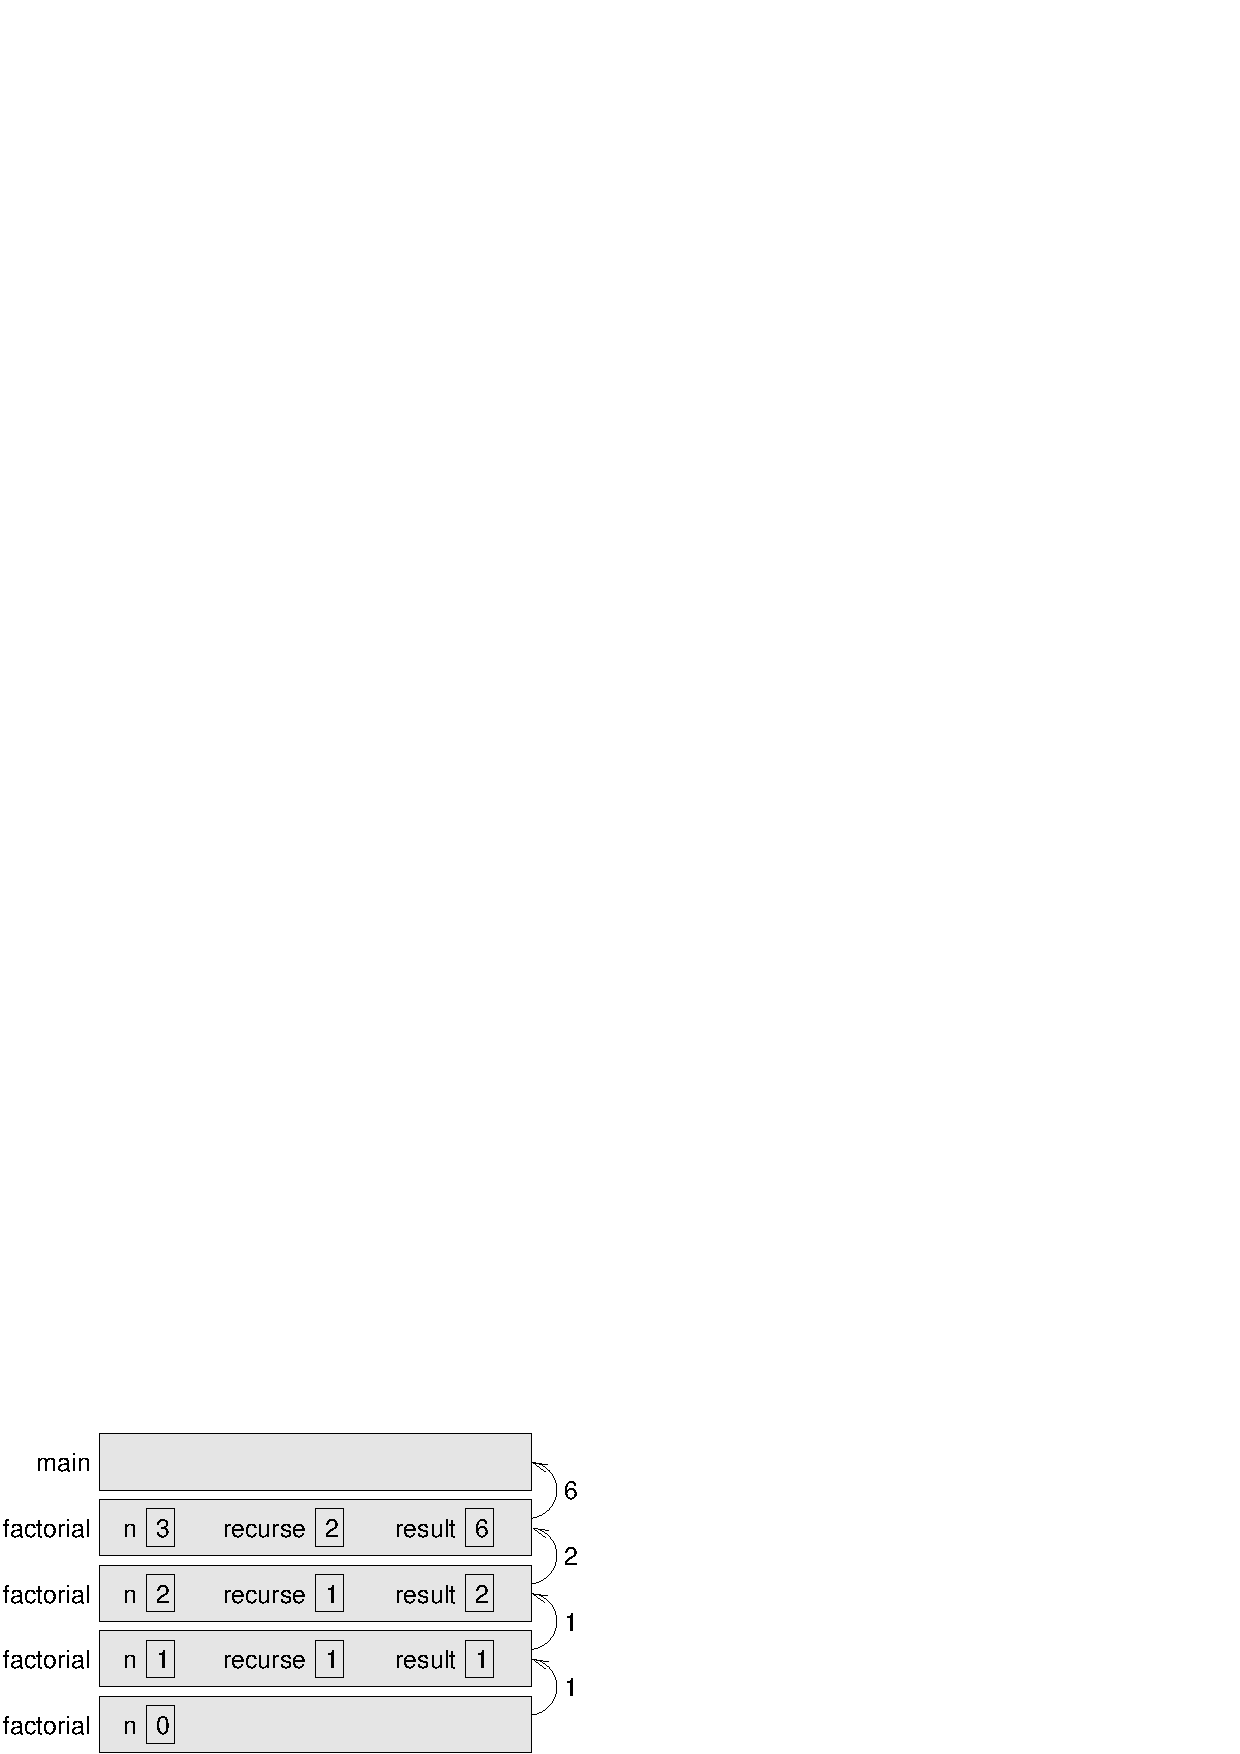
\includegraphics{figs/stack3.pdf}
\caption{Stack diagram for the \java{factorial} method.}
\label{fig:stack3}
\end{center}
\end{figure}


\section{Leap of faith}
\label{leap of faith}

\index{leap of faith}

Following the flow of execution is one way to read programs, but it can quickly become disorienting.
An alternative to drawing lengthy stack diagrams is simply a ``leap of faith.''
When you come to a method invocation, instead of following the flow of execution, you {\em assume} that the method works correctly and returns the appropriate value.

In fact, you are already practicing this leap of faith when you use methods in the Java library.
When you invoke {\tt Math.cos} or {\tt System.out.println}, you don't examine the implementations of those methods.
You just assume that they work properly.

You should apply the same reasoning to your own methods.
For example, in Section~\ref{boolean} we wrote a method called {\tt isSingleDigit} that determines whether a number is between 0 and 9.
Once we convince ourselves that this method is correct---by testing and examination of the code---we can use the method without ever looking at the code again.

The same is true of recursive programs.
When you get to the recursive call, instead of following the flow of execution you should {\em assume} that the recursive invocation works.
For example, ``Assuming that I can find the factorial of $n-1$, can I compute the factorial of $n$?''
Yes you can, by multiplying by $n$.

Of course, it is strange to assume that the method works correctly when you have not even finished writing it; that's why it's called a leap of faith!


\section{One more example}
\label{fibonacci}

\index{fibonacci}

Another common example of recursively-defined mathematical functions is the Fibonacci sequence, which has the following definition:

\vspace{-1ex}
\begin{eqnarray*}
&& fibonacci(1) = 1 \\
&& fibonacci(2) = 1 \\
&& fibonacci(n) = fibonacci(n-1) + fibonacci(n-2);
\end{eqnarray*}
\vspace{-1ex}

Translated into Java, this function is simply:

\begin{code}
    public static int fibonacci(int n) {
        if (n == 1 || n == 2) {
            return 1;
        } else {
            return fibonacci(n - 1) + fibonacci(n - 2);
        }
    }
\end{code}

If you try to follow the flow of execution here, even for small values of \java{n}, your head will explode.
But according to the leap of faith, if we assume that the two recursive invocations work correctly, then it is clear that we get the right result by adding them together.


\section{Testing with JUnit}

To convince yourself that anything works, you should always test it.
The first ten Fibonacci numbers are 1, 1, 2, 3, 5, 8, 13, 21, 34, and 55.
We can write a simple \java{main} method to test the \java{fibonacci} method.

\begin{code}
    public static void main(String[] args) {
        if (fibonacci(1) != 1) {
            System.err.println("1 is incorrect");
        }
        // copy that if statement nine more times
    }
\end{code}

JUnit is a framework that helps automate and standardize this process (see \url{http://junit.org/}).
The basic pattern is very simple:

\begin{itemize}
\item For every class \java{X} there is a companion class named \java{XTest} that is responsible for testing the class.
\item For every method \java{m} there is a companion method \java{testM} that is responsible for testing the method.
\end{itemize}

For example, the \java{fibonacci} method in the previous section belongs to a class named \java{Series}.
Here are the corresponding test class and test method:

\begin{code}
import junit.framework.TestCase;

public class SeriesTest extends TestCase {
    
    public void testFibonacci() {
        assertEquals(1, Series.fibonacci(1));
        assertEquals(1, Series.fibonacci(2));
        assertEquals(2, Series.fibonacci(3));
        assertEquals(3, Series.fibonacci(4));
        // six more assertEquals statements
    }
    
}
\end{code}

Since JUnit is industry strength, it uses some Java language features we have not yet studied in this book (e.g., \java{extends}).
However, it's easy to get started by writing simple test methods.
In DrJava, you can select ``File $>$ New JUnit Test Case'' from the menu to generate the required \java{import} and \java{extends} code.

JUnit provides a family of overloaded \java{assert} methods.
In the example above, \java{assertEquals} compares expected values (e.g., 1) with actual values (e.g., what \java{fibonacci} returns).
If an assertion fails, it displays an error showing the values that did not match.
This code is more concise than writing your own \java{if} statements and \java{System.err} messages.

To run JUnit directly from DrJava, click the {\tt Test} button on the toolbar.
If all your test methods pass, you will see a green rectangle on the lower right.
Otherwise, it will take you directly to the first assertion that failed.


\section{Vocabulary}

\begin{description}

\term{return type}
The part of a method declaration that indicates what type of value the method returns.

\term{return value}
The value provided as the result of a method invocation.

\term{void}
A special return type indicating the method does not return a value.

\term{temporary variable}
A variable that is short-lived, often declared for debugging purposes.

\term{dead code}
Part of a program that can never be executed, often because it appears after a {\tt return} statement.

\term{stub}
A placeholder for an incomplete method so that the class will compile.

\term{scaffolding}
Code that is used during program development but is not part of the final version.

\term{overloading}
Defining more than one method with the same name but different parameters.
%When you invoke an overloaded method, Java knows which version to use by looking at the arguments you provide.

\term{Turing complete}
A programming language that can implement any theoretically possible algorithm.

\term{factorial}
The product of all the integers up to and including a given integer.

\end{description}


\section{Exercises}

\begin{exercise}
\label{ex.isdiv}

Write a method named \java{isDivisible} that takes two integers, \java{n} and \java{m}, and that returns \java{true} if \java{n} is divisible by \java{m}, and \java{false} otherwise.
\end{exercise}

\begin{exercise}
If you are given three sticks, you may or may not be able to arrange them in a triangle.
For example, if one of the sticks is 12 inches long and the other two are one inch long, you will not be able to get the short sticks to meet in the middle.
For any three lengths, there is a simple test to see if it is possible to form a triangle:

\begin{quote}
``If any of the three lengths is greater than the sum of the other two, then you cannot form a triangle.''
\end{quote}

Write a method named \java{isTriangle} that takes three integers as arguments and returns either \java{true} or \java{false}, depending on whether you can or cannot form a triangle from sticks with the given lengths.
The point of this exercise is to use conditional statements to write a value method.
\end{exercise}

\begin{exercise}
\label{ex.multadd}

Many computations can be expressed more concisely using the ``multadd'' operation, which takes three operands and computes \java{a * b + c}.
Some processors even provide a hardware implementation of this operation for floating-point numbers.

\begin{enumerate}

\item Create a new program called {\tt Multadd.java}.

\item Write a method called {\tt multadd} that takes three {\tt doubles} as parameters and that returns \java{a * b + c}.

\item Write a \java{main} method that tests \java{multadd} by invoking it with a few simple parameters, like \java{1.0, 2.0, 3.0}.

\item Also in \java{main}, use \java{multadd} to compute the following values:

\begin{eqnarray*}
& \sin \frac{\pi}{4} + \frac{\cos \frac{\pi}{4}}{2} & \\
& \log 10 + \log 20 &
\end{eqnarray*}

\item Write a method called \java{yikes} that takes a double as a parameter and that uses \java{multadd} to calculate:

\begin{eqnarray*}
x e^{-x} + \sqrt{1 - e^{-x}}
\end{eqnarray*}

HINT: The Math method for raising $e$ to a power is \java{Math.exp}.

\end{enumerate}

In the last part, you get a chance to write a method that invokes a method you wrote.
Whenever you do that, it is a good idea to test the first method carefully before you start working on the second.
Otherwise, you might find yourself debugging two methods at the same time, which can be difficult.

One of the purposes of this exercise is to practice pattern-matching: the ability to recognize a specific problem as an instance of a general category of problems.
\end{exercise}

\begin{exercise}
What is the output of the following program?

\begin{code}
    public static void main(String[] args) {
        boolean flag1 = isHoopy(202);
        boolean flag2 = isFrabjuous(202);
        System.out.println(flag1);
        System.out.println(flag2);
        if (flag1 && flag2) {
            System.out.println("ping!");
        }
        if (flag1 || flag2) {
            System.out.println("pong!");
        }
    }

    public static boolean isHoopy(int x) {
        boolean hoopyFlag;
        if (x % 2 == 0) {
            hoopyFlag = true;
        } else {
            hoopyFlag = false;
        }
        return hoopyFlag;
    }

    public static boolean isFrabjuous(int x) {
        boolean frabjuousFlag;
        if (x > 0) {
            frabjuousFlag = true;
        } else {
            frabjuousFlag = false;
        }
        return frabjuousFlag;
    }
\end{code}

The purpose of this exercise is to make sure you understand logical operators and the flow of execution through value methods.
\end{exercise}

% TODO(CSM): Remove this exercise? It's very similar to the example in the chapter.
%
%\begin{exercise}
%The distance between two points $(x_1, y_1)$ and $(x_2, y_2)$ is
%
%\[ Distance = \sqrt{(x_2 - x_1)^2 +(y_2 - y_1)^2} \]
%
%Write a method named {\tt distance} that takes four doubles as parameters---{\tt x1}, {\tt y1}, {\tt x2} and {\tt y2}---and that prints the distance between the points.
%
%You should assume that there is a method named {\tt sumSquares} that calculates and returns the sum of the squares of its arguments.
%For example:
%
%\begin{code}
%    double x = sumSquares(3.0, 4.0);
%\end{code}
%
%would assign the value {\tt 25.0} to {\tt x}.
%
%The point of this exercise is to write a new method that uses an existing one.
%You should write only one method: {\tt distance}.
%You should not write {\tt sumSquares} or {\tt main}, and you should not invoke {\tt distance}.
%\end{exercise}

\newpage

\begin{exercise}
The point of this exercise is to use a stack diagram to understand the execution of a recursive program.

\begin{code}
public class Prod {

    public static void main(String[] args) {
        System.out.println(prod(1, 4));
    }

    public static int prod(int m, int n) {
        if (m == n) {
            return n;
        } else {
            int recurse = prod(m, n-1);
            int result = n * recurse;
            return result;
        }
    }
}
\end{code}

\begin{enumerate}

\item Draw a stack diagram showing the state of the program just before the last instance of \java{prod} completes.
What is the output of this program?

\item Explain in a few words what \java{prod} does.

\item Rewrite \java{prod} without using temporary variables \java{recurse} and \java{result}.

\end{enumerate}
\end{exercise}

\begin{exercise}
The purpose of this exercise is to translate a recursive definition into a Java method.
The Ackermann function is defined for non-negative integers as follows:
\begin{eqnarray*}
A(m, n) = \begin{cases}
              n+1 & \mbox{if } m = 0 \\
        A(m-1, 1) & \mbox{if } m > 0 \mbox{ and } n = 0 \\
A(m-1, A(m, n-1)) & \mbox{if } m > 0 \mbox{ and } n > 0.
\end{cases}
\end{eqnarray*}

Write a method called \java{ack} that takes two \java{int}s as parameters and that computes and returns the value of the Ackermann function.

Test your implementation of Ackermann by invoking it from \java{main} and printing the return value.
Note the return value gets very big very quickly.
You should try it only for small values of $m$ and $n$ (not bigger than 3).
\end{exercise}

% TODO(CSM): move to strings and things chapter?

\begin{exercise}
Create a program called {\tt Recurse.java} and type in the following methods:

\begin{code}
    // first: returns the first character of the given String
    public static char first(String s) {
        return s.charAt(0);
    }

    // last: returns a new String that contains all but the
    // first letter of the given String
    public static String rest(String s) {
        return s.substring(1, s.length());
    }

    // length: returns the length of the given String
    public static int length(String s) {
        return s.length();
    }
\end{code}

\begin{enumerate}

\item Write some code in \java{main} that tests each of these methods.
Make sure they work, and make sure you understand what they do.

\item Write a method called \java{printString} that takes a String as a parameter and that prints the letters of the String, one on each line.  It should be a \java{void} method.

\item Write a method called \java{printBackward} that does the same thing as \java{printString} but that prints the String backward (again, one character per line).

\item Write a method called \java{reverseString} that takes a String as a parameter and that returns a new String as a return value.
The new String should contain the same letters as the parameter, but in reverse order.

\begin{code}
    String backwards = reverseString("Allen Downey");
    System.out.println(backwards);
\end{code}

For example, the output of the above code should be:

\begin{stdout}
yenwoD nellA
\end{stdout}

\end{enumerate}
\end{exercise}

\begin{exercise}
\label{ex.power}
Write a recursive method called \java{power} that takes a double \java{x} and an integer \java{n} and that returns $x^n$.

Hint: a recursive definition of this operation is $x^n = x \cdot x^{n-1}$.
Also, remember that anything raised to the zeroeth power is 1.

Optional challenge: you can make this method more efficient, when \java{n} is even, using $x^n = \left( x^{n/2} \right)^2$.
\end{exercise}

\begin{exercise}
\label{gcd}
(This exercise is based on page 44 of Ableson and Sussman's {\em Structure and Interpretation of Computer Programs}.)

The following technique is known as Euclid's Algorithm, because it appears in Euclid's {\em Elements} (Book 7, ca.~300 BC).
It may be the oldest recorded nontrivial algorithm.
%\footnote{For a definition of ``algorithm'', jump ahead to Section~\ref{algorithm}.}  NOW IN CHAPTER 1

The process is based on the observation that, if $r$ is the remainder when $a$ is divided by $b$, then the common divisors of $a$ and $b$ are the same as the common divisors of $b$ and $r$.
Thus we can use the equation:

\[ gcd(a, b) = gcd(b, r) \]

to successively reduce the problem of computing a GCD to the problem of computing the GCD of smaller and smaller pairs of integers.
For example,

\[ gcd(36, 20) = gcd(20, 16) = gcd(16, 4) = gcd(4, 0) = 4 \]

implies that the GCD of 36 and 20 is 4.
It can be shown that for any two starting numbers, this repeated reduction eventually produces a pair where the second number is 0.
Then the GCD is the other number in the pair.

Write a method called \java{gcd} that takes two integer parameters and that uses Euclid's algorithm to compute and return the greatest common divisor of the two numbers.
\end{exercise}


\end{document}
